\chapter{Document Oriented Databases}
\section{Introduction}
\chapterauthor{Andreas Fuchs, Alex Schäfer, Cathleen Schmalfuß}
Document store databases are one representative of NoSQL databases. They are commonly referred to by either document store database or document-oriented database, more rarely aggregated database is being used. Instead of focusing on relationships the focus for this type lies on structuring data in more natural or logical ways \parencite{mongodb2019}. In short, it uses \textquote[\parencite{ian2016}]{a document-oriented model to store data}. 

\subsection{Document Oriented Databases explained}
Each record is made of a single document, including the record itself and all associated data \parencite{ian2016}\parencite{amazonNoSql}. This puts a record into a single logical unit, making it easier to manage since all related data is kept together at all times - Even in case of distributed data across multiple servers. This also leads to an increase in performance since a logical unit can be \textquote[\parencite{mongodb2019}]{read contiguously off disk}. Another advantage follows the possible simplification of the application logic. With this way of processing and storing data, objects can be directly transformed into a document instead of translating them into SQL queries first \parencite{mongodb2019}  \parencite{amazonNoSql}. Objects can be stored \enquote{as they are}, with no need to force them into a structure of a static table, especially if there is only one instance of that object in use. This leads to an overall ease of storing unstructured data, since document store documents can contain all keys and values as needed without complex model transformations or adaptions \parencite{mongodb2019}. Additionally changes to the object model can easily be tracked and displayed. All iterations of a single object instance and their ever changing flexible attributes may be stored without transformation issues and database table adaptation. Since the document data structures can vary from document to document  \parencite{amazonNoSql}, it increases overall flexibility in the development process and reduces overhead of finding a static structure that fits all data equally. Document store databases are often described as \textquote[\parencite{amazonNoSql}]{designed to store semi structured data}, because even though data is less structured than in a classic relationship model, keys and values still provide some structure, even though an overall much more adaptable one.

\subsection{Document Oriented Databases over the Years}
A ranking from March 2019 shows the top 11 document store databases in use today \parencite{dbEngineRankingPopularity}. db-engines.com was consulted for \autoref{docoriented:figure:Ranking} and \autoref{docoriented:figure:Development}. MongoDB is still leading on rank 1 of the most popular document oriented databases, same as it did for the last three years. \autoref{docoriented:figure:Ranking} shows that overall only very small changes happened in the total top 10 in the last three years. RethinkDB moved down to 11 and Google Cloud Datastore instead made it up to 9. CouchDB and Microsoft Azure Cosmos DB bested over each other in place 4 and 5. Other than that the document oriented database market has been very quiet. This proves how a handful of document oriented database systems already claimed leading roles on the market.
\begin{figure}
    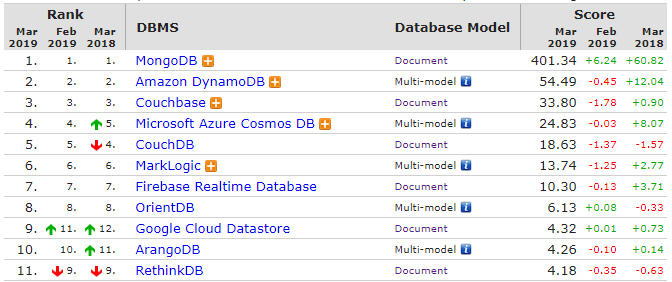
\includegraphics[width=\textwidth]{img/dbRanked.png}
    \caption{Ranking of documented oriented databases}
    \label{docoriented:figure:Ranking}
\end{figure}
Overall not many changes happened in the ranking over that last three years. The development and establishment of these databases can therefore be seen as a longer running process. Three years is a short time frame to retrace the whole market development. To demonstrate how the top 5 as well as RethinkDB (currently 11) established themselves over a longer period consider \autoref{docoriented:figure:Development}. It provides insight in the development of the document oriented database market and the popularity of the leading five products in ranking since 2013 \parencite{dbEngineRankingPopularity}. 

\begin{figure}
    \centering
    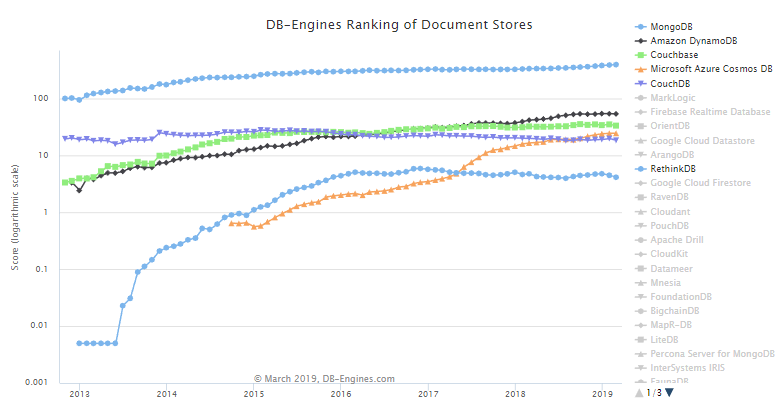
\includegraphics[width=\textwidth]{img/dbRankedTrend.png}
    \caption{Development of the document oriented database market}
    \label{docoriented:figure:Development}
\end{figure}

Ever since 2013 MongoDB has had a leading role. However, the top 3 of today were not as set back then. Further \autoref{docoriented:figure:Development} finally provides a bit more insight over the development of several products over time. CouchDB especially, once second to MongoDB, moved down to rank 5, while Amazon DynamoDB made a name for itself and claimed that second rank. Even though RethinkDB was recently overtaken by Microsoft Azure Cosmos DB it has an astonishing increase in popularity considering its small beginning back in 2013. So in the long run things weren't as set as they have been over the last three years. The historic development of the products and especially the features added, which lead to a sometimes rather steep ascend in popularity, are relevant still.

\subsection{Comparison relational database management systems (RDMS)}
\label{docoriented:section:postalcodes}
Before going into details of specific document store databases this chapter will focus on comparing classical relational database management systems (RDMS) with the new concept of document store databases. This will provide a closer insight into the structure and working of document store databases as well as its general advantages and disadvantages not only in direct comparison.

As the name suggests RDMS focus primarily on relationships. Properties of a data set are spread across different tables and linked using primary and foreign keys to reference and link information. This means a reference - mostly given as a foreign key pointing to the primary key of the needed information entry - can be reused multiple times in different tables across the database. Master data may be used and reused as often as needed, a simple example of a list providing such master data would be a list hosting all relevant postal codes for an application dealing with addresses or shipping in an area. This also means that the data related to a set is spread across the database, needing to be retrieved via the foreign key from different tables. To go over the main differences between such a table and relationship based setup and the document oriented approach, consider the following points.
\subsubsection{Tables}
For RDMS tables are in the centre of the system. Different tables may be linked to describe relationships and reference data. Strictly speaking a single record is described as a row in a table, additional information may be supplied from a different table. All records are bound to this static structure and the columns given in this record table. Therefore records of the same table need to share the same columns to describe their properties.

In the document store based system a single document describes all data related to this entry. No reference to other documents are necessarily made. Seeing that a document always has an unique key to identify it, relations can be technically set up.

Depending on the focus, either the data as such or the common relationships data entries have, a document store or a RDMS brings advantages. It is far easier to group entries in a table sorting by a foreign key reference to for example collect all entries linked to a specific postal code. It is however easier using a document store database to store data which not necessarily shares the exact same properties, therefore cannot be mapped into a strict column based format.
\subsubsection{Schemas}
As the table based design suggests the RDMS is very strict. The schema how columns are used to describe an entry and what data needs to be gathered from another table must be known from the beginning. There is no flexible adaptation depending on the data provided. A record either has all the properties asked for by the schema or null values may be inserted, leading to the question whether the information was unknown, missing or not provided due to an error.

The document store based system can manage documents that differ. This means two entries do not necessarily have to have the same structure or even data attributes \parencite{amazonNoSql}\parencite{objelean}. A common example is a web form where a user can provide some of their details optionally. A RDMS entry would have columns for every property, leaving fields empty if the information is not provided. A document on the other hand stores only the information given.

Advantages depend on the use case scenario. In some cases, especially towards the end of development when a fixed data schema has been agreed on, the very conventional approach of using a SQL database may work just fine. However, especially during development of an application, when data processed is still being explored and especially the difference of data sets (objects) is key to understanding it, a document store may offer more flexibility.
\subsubsection{Scalability}
Relationship databases scale well vertically, the addition of memory or storage to the machine increases the performance. However vertical scaling has a limit, which leads to the need to scale horizontally to further increase performance. The horizontal implementation of RDMS is a complex process that asks for redundancy and different strategies to keep data across the horizontal landscape consistent.

A document based system is much easier to spread horizontally \parencite{ian2016}\parencite{objelean}. Each entry is in itself complete and can be stored across a large landscape since no additional information is linked or needs to be gathered from a possible far away source. The process of storing data across such a landscape is called \enquote{sharding} \parencite{ian2016}.
\subsubsection{Relationships}
Relationships are the central idea of RDMS while tables are the central storage form to implement them. The idea is to associate data entries with different ones to capture relationships and common links. Again, remember the example of the reusable postal code column from section \ref{docoriented:section:postalcodes}.

A document store based system does not provide means to implement this idea. Here the central idea is to keep all data together that is needed to describe a record. If relations are indeed still needed, this needs to happen at application level \parencite{ian2016} using the unique keys that identify the documents (records).
\subsubsection{Querying}
Relational databases tend to use SQL (structured query language) to query their tables and records. Document store databases may support SQL statements, but most are queried with different languages \textquote[\parencite{ian2016}]{such as XQuery, XSLT, SPARQL, Java, JavaScript, Python}  for example.

There are no strict advantages over what query language is being used. However, one might consider the general performance of retrieving records from the database or the complexity of the query statements needed to do common actions (read, write, update, delete) against the specific database with its specific query language.
